
In this section we outline the estimated impact of MW changes on rent and house prices. We first how show the estimated impact of MW changes - as captured by \autoref{eq:main_ziplevel} - [ADD INTRO RESULTS]. As introduced in \autoref{sec:empirical_strategy}, when restricting the sample to have only one event per unit, identification is only reached up to a linear trend. We then present results for the first different specification: the estimated \textit{average treatment effect} decreases to XX. 

\subsection{An event-study specification}\label{subsec:results/event-study}

In this subsection, we present estimation results using median rents as our dependent variable. We focus on the median rent per square foot for single family houses and condos as this is the most populated time series in the Zillow rent data. [ADD ZILLOW DATA TABLE TO APPENDIX?]. \\

\autoref{fig:event_level_sal_6} plots the relative event coefficients from \autoref{eq:main_ziplevel}, where the dependent variable is the zipcode-level median rent per square foot for single family houses, condos and coop housing. In this initial setting, an event is considered to be a MW change of at least $\$0.5$.  

\begin{figure}[h!]
    \centering
    \caption{Effects of a MW change of at least \$0.5 on single family rent per square foot (in dollars).}
    \scalebox{0.45}{
    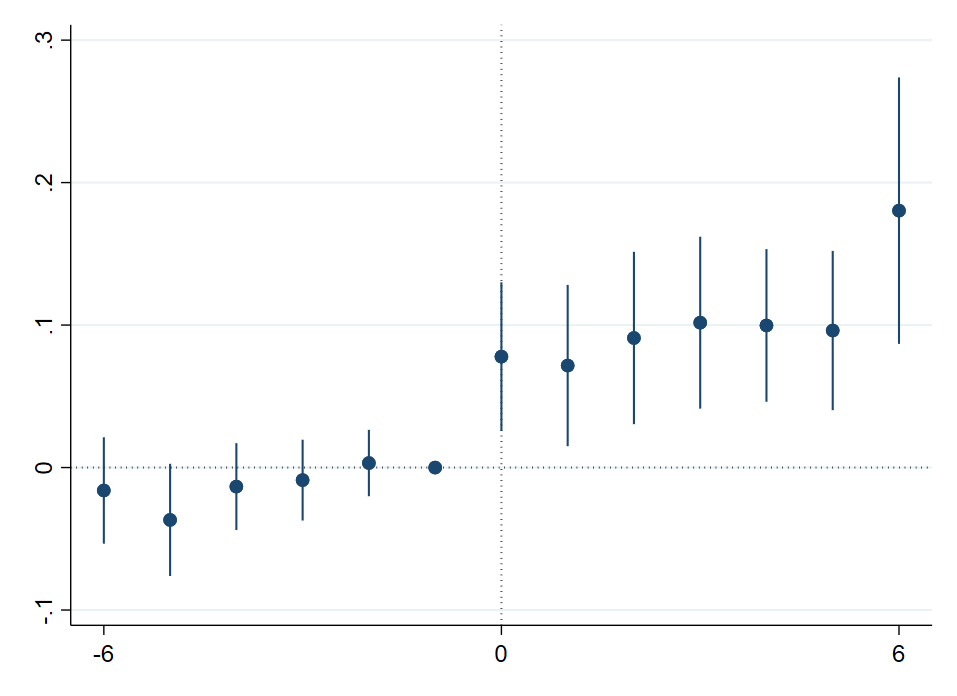
\includegraphics{analysis/event_study/output/last_rentpsqft_sfcc_w6.png}
    }
    \subcaption*{\textit{Note}: The figure shows the estimated $\hat{\delta}_{t+k}$ coefficients from the baseline specification. For each zipcode, we  add the sum of unused events and county-level seasonality as additional controls ($X_{jt}$). Avearage MW change: $\$0.8$. Standard errors are clustered at the zipcode level.}
    \label{fig:event_level_sal_6}
\end{figure}

The figure shows a rather flat and not statistically significant pre-trend followed by a immediate impact of around ten cents on rent that remains stable in the following months. 
To better understand the magnitude of such effect, notice that in the present specification the average increase of the MW change is of $\$0.8$. This implies that, for a family of 2 minimum wagers woring 40 hours a week, this change represents an increase on the family income of approximately \$278.4.\footnote{The average month has 4.35 weeks.} Assuming that this representative single family consumes 1500 square feet of housing, the implied increase in monthly rent is of about \$150, which implies an on-impact pass-through from the MW change to rents of 53.9\%. If assuming that the treatment effect is given by averaging the 7 post event coefficient, then the implies pass-through is of about 64.4\%.

First note that, taken at face value this number seems slightly high given that the median US rent requires 28.4\% of the median incomes \parencite{bi}. However, a household with 2 full time minimum wagers making, for example, the federal minimum wage of \$7.25 will have an annual income of \$30276, only slightly above half of the median US household income of \$59430 in 2015, which suggests that the estimated pass-through is plausible. 

Second, we check the robustness of this result by changing the prominence of the MW changes. Specifically, In \autoref{appfig:event_level_robustness6} we use MW changes that comply to our sample criterion (explained in section 2) and are of at least \$0.25 and of at least \$0.75 instead of \$0.5. we show how, as we increase the size of the MW changes to be considered as an event, the estimated effect becomes more persistent in the periods following the change. 

To get a more precise estimate of the impact on low-income households, for each of the event definitions we bootstrap, clustering at the zipcode level, the whole computation of the pass-through (assuming that the relevant per square foot effect is the average of the post event coefficients). The results are presented in Table \ref{tab:bootstrap_table}, where the column (2) corresponds to Figure \ref{fig:event_level_sal_6}. Note that we compute the implied pass-through for 3 different housing size - 1000, 1500, and 2000 square feet - in order to cover a plausible range of values for the average rental of a single family with 2 MW earners. Finally, note that as in any event-study, we are using only the zipcodes that have at least one MW change in our period. The estimated pass-throughs are all significantly different from zero: looking at the first row of \autoref{tab:bootstrap_table} we can see how rents show an average increase of around $0.7$ percent across MW changes of various strength. 


\begin{table}[h!]
    \centering
    \caption{Bootstrap estimates of the main objects of interest}
    \resizebox{\textwidth}{!}{
    {
\def\sym#1{\ifmmode^{#1}\else\(^{#1}\)\fi}
\begin{tabular}{l*{3}{c}}
\hline\hline
            &\multicolumn{1}{c}{(1)}        &\multicolumn{1}{c}{(2)}        &\multicolumn{1}{c}{(3)}        \\
            &\multicolumn{1}{c}{MW changes of at least \$0.25}&\multicolumn{1}{c}{MW changes of at least \$0.5}&\multicolumn{1}{c}{MW changes of at least \$0.75}\\
\hline
Rent increase per square feet&                0.0139         &                0.0730\sym{*}  &                0.0687\sym{***}\\
            &     [-0.00716,0.0350]         &        [0.0136,0.132]         &        [0.0313,0.106]         \\
[1em]
Total rent increase (assuming 1000 square feet)&                 13.93         &                 72.97\sym{*}  &                 68.73\sym{***}\\
            &        [-7.161,35.03]         &         [13.57,132.4]         &         [31.34,106.1]         \\
[1em]
Total rent increase (assuming 1500 square feet)&                 20.90         &                 109.5\sym{*}  &                 103.1\sym{***}\\
            &        [-10.74,52.54]         &         [20.35,198.6]         &         [47.01,159.2]         \\
[1em]
Total rent increase (assuming 2000 square feet)&                 27.86         &                 145.9\sym{*}  &                 137.5\sym{***}\\
            &        [-14.32,70.05]         &         [27.13,264.8]         &         [62.69,212.2]         \\
[1em]
Increase in income of a household with 2 full time minimum wages&                 208.8\sym{***}&                 274.9\sym{***}&                 424.6\sym{***}\\
            &         [199.8,217.8]         &         [266.3,283.5]         &         [406.6,442.5]         \\
[1em]
Implied passthrough from MW to rents (assuming 1000 square feet)&                0.0667         &                 0.265\sym{*}  &                 0.162\sym{***}\\
            &       [-0.0352,0.169]         &        [0.0500,0.481]         &        [0.0740,0.250]         \\
[1em]
Implied passthrough from MW to rents (assuming 1500 square feet)&                 0.100         &                 0.398\sym{*}  &                 0.243\sym{***}\\
            &       [-0.0528,0.253]         &        [0.0751,0.721]         &         [0.111,0.375]         \\
[1em]
Implied passthrough from MW to rents (assuming 2000 square feet)&                 0.133         &                 0.531\sym{*}  &                 0.324\sym{***}\\
            &       [-0.0704,0.337]         &         [0.100,0.962]         &         [0.148,0.499]         \\
\hline
Minimum MW change&                               &                               &                               \\
Average MW change&                    .6         &                   .79         &                  1.22         \\
Maximum MW change&                               &                               &                               \\
Number of zipcode-months&                 59899         &                 36535         &                 30893         \\
Number of Zipcodes&                   572         &                   353         &                   299         \\
Number of bootstrap repetitions&                   181         &                   178         &                   176         \\
\hline\hline
\end{tabular}
}

    }
    \subcaption*{\textit{Notes:} Square brackets display the 95\% bootstrapped confidence intervals. Income computations are done assuming 2 MW earners.}
    \label{tab:bootstrap_table}
\end{table}


Next, we highlight the importance of allowing for flexible year-month fixed effects that are specific to the county. We highlight how this is possible since we are focusing on zipcode level variation, and we clarify the importance of it by introducing a comparison with a simpler specification: Figure \ref{fig:event_level_2way} presents an event study plot analogous to Figure \ref{fig:event_level_sal_6} but using a simple two-way fixed effect specification, which in our case corresponds to zipcode and year-month fixed effects. In such case, all variation across time and zipcodes ends up being used to estimate the relative event coefficients. This however may cause the model to be misspecified if, for example, different states or counties or MSAs were follwing different time trends in rent prices, as it is probably the case. In particular, as within zipcode variation is not "de-trended", the relative event coefficients will be much harder to estimate as they will be confounded by such trend. \\

\begin{figure}[h!]
    \centering
    \caption{Two-way fixed effects specification. Effects of a MW change of at least \$0.5 on single family rent per square foot (in dollars). Standard errors are clustered at the zipcode level.}
    \label{fig:event_level_2way}
    \scalebox{0.45}{
    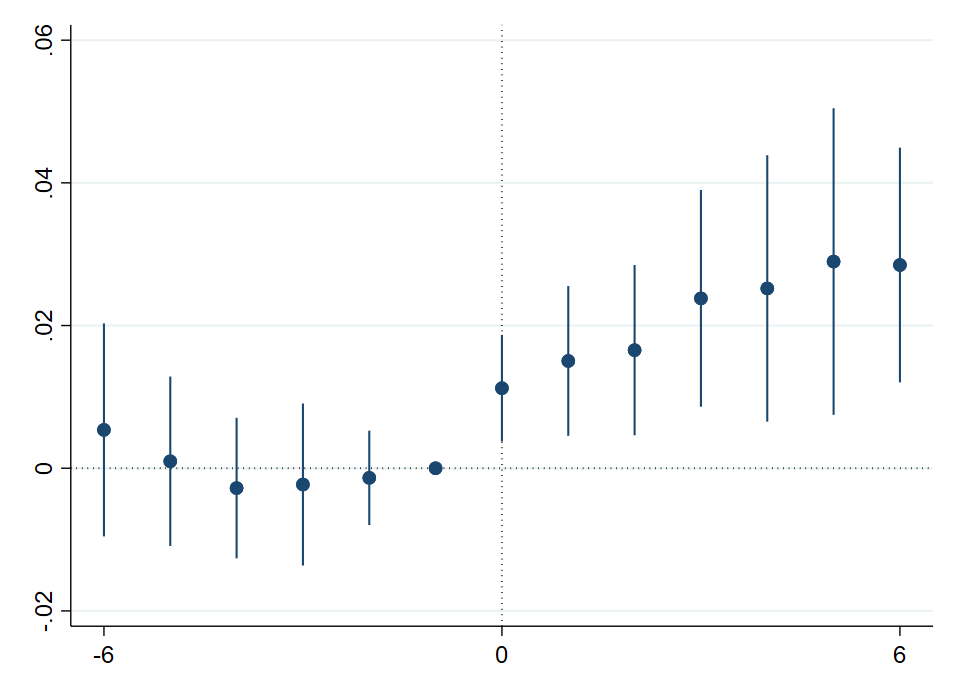
\includegraphics{analysis/event_study/output/two_way_last_medrentpricepsqft_sfcc6.png}
    }
    \subcaption*{\textit{Notes:} The figure shows the estimated $\hat{\delta}_{t+k}$ coefficients from two-way fixed effect specification at the zipcode-month level. Average MW change: $\$0.8$. Standard errors are clustered at the zipcode level.}
\end{figure}

In fact, we see that estimation of the relative coefficients is much noisier and lower in magnitude. The within variation R-squared (the percentage of the within variation in the data explained by the model) is of 0.0066. When allowing for county-specific time fixed effects and county-specific calendar months (to allow for flexible seasonality patterns) that were infeasible under the specifications in the previous literature we get the results shown in \ref{fig:event_level_sal_6} and a within variation R-squared of 0.0779, so that we are able to explain 12 times more the observed within zipcode variation. These results suggest that county-specific year-month and seasonal month variation are important determinants of monthly rent at the local level above and beyond what a two way fixed effects model could capture.

With the last result of this subsection, we show the importance of a granular analysis of MW changes by looking at the implications of aggregating our zipcode-month data at the county-quarter level\footnote{In order to use the data in the same unit as \textcite{tidemann2018mw,yamagishi2019minimum} we should have aggregated at the county-year. However, that involves dealing with overlap in the events for each county as we have many MW changes on subsequent years. Therefore, we aggregated the data at the county-quarter under the thought that we can only do better than at the county-year.}. Figure \ref{fig:event_level_county2way} plots the relative event coefficients for a two-way fixed effect specification at the county-quarter, for a window of 2 quarters around MW changes of at least \$0.5. Similar to \textcite{tidemann2018mw} results are very imprecise and point estimates are, if anything, negative. 

\begin{figure}[h!]
    \centering
    \caption{Two-way fixed effects county-quarter specification}
    \label{fig:event_level_county2way}
    \scalebox{0.45}{
    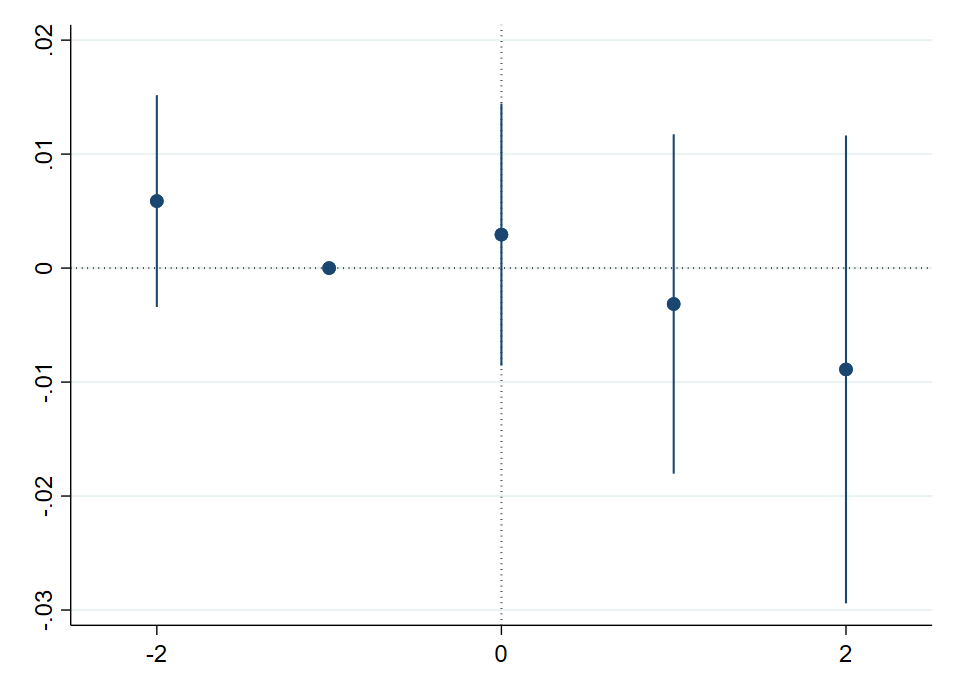
\includegraphics{analysis/event_study_county_quarter/output/last_rentpsqft_sfcc_w2.png}
    }
    \subcaption*{\textit{Notes:} The figure shows the effect of a MW change of at least \$0.5 on single family rent per square foot (in dollars). We plot the estimated coefficients from a two-way fixed effect specification at the county-quarter level. 
    Standard errors are clustered at the zipcode level.}
\end{figure}

\subsection{First-differences specification}\label{subsec:results/first-differences}




\subsection{Assessing magnitude of the effects}\label{subsec:results/magnitude}


